% Options for packages loaded elsewhere
\PassOptionsToPackage{unicode}{hyperref}
\PassOptionsToPackage{hyphens}{url}
%
\documentclass[
]{article}
\usepackage{amsmath,amssymb}
\usepackage{lmodern}
\usepackage{iftex}
\ifPDFTeX
  \usepackage[T1]{fontenc}
  \usepackage[utf8]{inputenc}
  \usepackage{textcomp} % provide euro and other symbols
\else % if luatex or xetex
  \usepackage{unicode-math}
  \defaultfontfeatures{Scale=MatchLowercase}
  \defaultfontfeatures[\rmfamily]{Ligatures=TeX,Scale=1}
\fi
% Use upquote if available, for straight quotes in verbatim environments
\IfFileExists{upquote.sty}{\usepackage{upquote}}{}
\IfFileExists{microtype.sty}{% use microtype if available
  \usepackage[]{microtype}
  \UseMicrotypeSet[protrusion]{basicmath} % disable protrusion for tt fonts
}{}
\makeatletter
\@ifundefined{KOMAClassName}{% if non-KOMA class
  \IfFileExists{parskip.sty}{%
    \usepackage{parskip}
  }{% else
    \setlength{\parindent}{0pt}
    \setlength{\parskip}{6pt plus 2pt minus 1pt}}
}{% if KOMA class
  \KOMAoptions{parskip=half}}
\makeatother
\usepackage{xcolor}
\usepackage[margin=1in]{geometry}
\usepackage{color}
\usepackage{fancyvrb}
\newcommand{\VerbBar}{|}
\newcommand{\VERB}{\Verb[commandchars=\\\{\}]}
\DefineVerbatimEnvironment{Highlighting}{Verbatim}{commandchars=\\\{\}}
% Add ',fontsize=\small' for more characters per line
\usepackage{framed}
\definecolor{shadecolor}{RGB}{248,248,248}
\newenvironment{Shaded}{\begin{snugshade}}{\end{snugshade}}
\newcommand{\AlertTok}[1]{\textcolor[rgb]{0.94,0.16,0.16}{#1}}
\newcommand{\AnnotationTok}[1]{\textcolor[rgb]{0.56,0.35,0.01}{\textbf{\textit{#1}}}}
\newcommand{\AttributeTok}[1]{\textcolor[rgb]{0.77,0.63,0.00}{#1}}
\newcommand{\BaseNTok}[1]{\textcolor[rgb]{0.00,0.00,0.81}{#1}}
\newcommand{\BuiltInTok}[1]{#1}
\newcommand{\CharTok}[1]{\textcolor[rgb]{0.31,0.60,0.02}{#1}}
\newcommand{\CommentTok}[1]{\textcolor[rgb]{0.56,0.35,0.01}{\textit{#1}}}
\newcommand{\CommentVarTok}[1]{\textcolor[rgb]{0.56,0.35,0.01}{\textbf{\textit{#1}}}}
\newcommand{\ConstantTok}[1]{\textcolor[rgb]{0.00,0.00,0.00}{#1}}
\newcommand{\ControlFlowTok}[1]{\textcolor[rgb]{0.13,0.29,0.53}{\textbf{#1}}}
\newcommand{\DataTypeTok}[1]{\textcolor[rgb]{0.13,0.29,0.53}{#1}}
\newcommand{\DecValTok}[1]{\textcolor[rgb]{0.00,0.00,0.81}{#1}}
\newcommand{\DocumentationTok}[1]{\textcolor[rgb]{0.56,0.35,0.01}{\textbf{\textit{#1}}}}
\newcommand{\ErrorTok}[1]{\textcolor[rgb]{0.64,0.00,0.00}{\textbf{#1}}}
\newcommand{\ExtensionTok}[1]{#1}
\newcommand{\FloatTok}[1]{\textcolor[rgb]{0.00,0.00,0.81}{#1}}
\newcommand{\FunctionTok}[1]{\textcolor[rgb]{0.00,0.00,0.00}{#1}}
\newcommand{\ImportTok}[1]{#1}
\newcommand{\InformationTok}[1]{\textcolor[rgb]{0.56,0.35,0.01}{\textbf{\textit{#1}}}}
\newcommand{\KeywordTok}[1]{\textcolor[rgb]{0.13,0.29,0.53}{\textbf{#1}}}
\newcommand{\NormalTok}[1]{#1}
\newcommand{\OperatorTok}[1]{\textcolor[rgb]{0.81,0.36,0.00}{\textbf{#1}}}
\newcommand{\OtherTok}[1]{\textcolor[rgb]{0.56,0.35,0.01}{#1}}
\newcommand{\PreprocessorTok}[1]{\textcolor[rgb]{0.56,0.35,0.01}{\textit{#1}}}
\newcommand{\RegionMarkerTok}[1]{#1}
\newcommand{\SpecialCharTok}[1]{\textcolor[rgb]{0.00,0.00,0.00}{#1}}
\newcommand{\SpecialStringTok}[1]{\textcolor[rgb]{0.31,0.60,0.02}{#1}}
\newcommand{\StringTok}[1]{\textcolor[rgb]{0.31,0.60,0.02}{#1}}
\newcommand{\VariableTok}[1]{\textcolor[rgb]{0.00,0.00,0.00}{#1}}
\newcommand{\VerbatimStringTok}[1]{\textcolor[rgb]{0.31,0.60,0.02}{#1}}
\newcommand{\WarningTok}[1]{\textcolor[rgb]{0.56,0.35,0.01}{\textbf{\textit{#1}}}}
\usepackage{graphicx}
\makeatletter
\def\maxwidth{\ifdim\Gin@nat@width>\linewidth\linewidth\else\Gin@nat@width\fi}
\def\maxheight{\ifdim\Gin@nat@height>\textheight\textheight\else\Gin@nat@height\fi}
\makeatother
% Scale images if necessary, so that they will not overflow the page
% margins by default, and it is still possible to overwrite the defaults
% using explicit options in \includegraphics[width, height, ...]{}
\setkeys{Gin}{width=\maxwidth,height=\maxheight,keepaspectratio}
% Set default figure placement to htbp
\makeatletter
\def\fps@figure{htbp}
\makeatother
\setlength{\emergencystretch}{3em} % prevent overfull lines
\providecommand{\tightlist}{%
  \setlength{\itemsep}{0pt}\setlength{\parskip}{0pt}}
\setcounter{secnumdepth}{-\maxdimen} % remove section numbering
\ifLuaTeX
  \usepackage{selnolig}  % disable illegal ligatures
\fi
\IfFileExists{bookmark.sty}{\usepackage{bookmark}}{\usepackage{hyperref}}
\IfFileExists{xurl.sty}{\usepackage{xurl}}{} % add URL line breaks if available
\urlstyle{same} % disable monospaced font for URLs
\hypersetup{
  pdftitle={SmartEDA},
  pdfauthor={Sayan Putatunda; Dayananda Ubrangala; Kiran Rama; Ravi Kondapalli; João Pedro Albino (Tradução)},
  hidelinks,
  pdfcreator={LaTeX via pandoc}}

\title{SmartEDA}
\usepackage{etoolbox}
\makeatletter
\providecommand{\subtitle}[1]{% add subtitle to \maketitle
  \apptocmd{\@title}{\par {\large #1 \par}}{}{}
}
\makeatother
\subtitle{Um pacote R para automatizar a Análise Exploratória de Dados}
\author{Sayan Putatunda \and Dayananda Ubrangala \and Kiran
Rama \and Ravi Kondapalli \and João Pedro Albino (Tradução)}
\date{07/01/2023}

\begin{document}
\maketitle

\hypertarget{introduuxe7uxe3o-anuxe1lise-exploratuxf3ria-de-dados}{%
\subsubsection{Introdução: Análise Exploratória de
Dados}\label{introduuxe7uxe3o-anuxe1lise-exploratuxf3ria-de-dados}}

Hoje em dia, vemos aplicações de Data Science em quase todos os
lugares.\\
Alguns dosaspectos mais bem destacados da ciência de dados são as várias
técnicas estatísticas e de aprendizado de máquina aplicadas na resolução
de problemas.\\
No entanto, qualquer atividade de ciência de dados começa com uma
\textbf{Análise Exploratória de Dados} (EDA - \emph{Exploratory Data
Analysis}).\\
O termo ``Análise Exploratória de Dados'' foi criado pelo matemático e
estatístico americano, John Tukey (SANDE, 2001). A EDA pode ser definida
como \emph{a arte e a ciência de realizar uma investigação inicial sobre
os dados} por meio de técnicas estatísticas e de visualizações que
possam trazer à tona os aspectos importantes nos dados e que podem ser
utilizados posteriormente no processo de análise (Tukey, 1977).\\
Na literatura estatística existem muitos estudos sobre EDA. Alguns dos
primeiros trabalhos realizados em Análise Exploratória de Dados (AED),
incluindo susa definição e o estabelecimento das técnicas básicas em AED
foram mostrados em Tukey (1977).\\
No entanto, muitos pesquisadores formularam diferentes definições de AED
ao longo dos anos.\\
Chon Ho (2010) introduziu a AED no contexto de mineração de dados e da
reamostragem com foco no reconhecimento de padrões, detecção de
agrupamentos (cluster) e na seleção de variáveis.\\
Ao longo dos anos, a AED tem sido utilizada em diversos tipos de
aplicações e em diferentes domínios, tais como: pesquisa em geociências
(Ma et al., 2017), avaliações baseadas em jogos (DiCerbo et al., 2015),
grupos de estudos clínicos (Konopka et al., 2018), dentre outros.\\
A AED pode ser categorizada em \textbf{técnicas estatísticas
descritivas} e \textbf{técnicas gráficas}. A primeira categoria abrange
várias técnicas estatísticas univariadas e multivariadas, enquanto a
segunda categoria compreende várias técnicas de visualização. Ambas as
técnicas são usadas para explorar e entender os padrões dos dados,
compreender as relações existentes entre as variáveis e, o mais
importante, gerar \textbf{insights} orientados por dados que podem ser
usados pelas partes interessadas (stakeholders) nos negócios. No
entanto, a AED requer muito esforço manual e também uma quantidade
substancial de esforço de codificação em um ambiente de programação como
o R (R Core Team, 2017). Existe uma grande necessidade de automação do
processo EDA, e isso nos motivou a desenvolver o pacote
\textbf{SmartEDA} e elaborar este artigo.

\hypertarget{principal-funcionalidade}{%
\subsubsection{Principal
Funcionalidade}\label{principal-funcionalidade}}

O pacote SmartEDA seleciona automaticamente as variáveis e executa as
funções estatisticas descritivas afins.\\
Além disso, também analisa o valor da informação, o peso da evidência,
tabelas personalizadas, estatísticas resumidas e executa técnicas
gráficas tanto para dados numéricos quanto categóricos.\\
Algumas das vantagens mais importantes do pacote SmartEDA são que ele
pode ajudar na aplicação de ponta a ponta do processo EDA sem ter que
lembrar os diferentes nomes de pacotes em R, escrever longos scripts em
R, e nenhum esforço manual é necessário para preparar o relatório EDA e,
finalmente, automaticamente categorizar as variáveis no tipo de dados
correto (ou seja, caractere, numérico, Fator e mais) com base nos dados
de entrada.\\
Assim, os principais benefícios do SmartEDA estão na economia de tempo
de desenvolvimento, menor percentual de erros e reprodutibilidade. Além
disso, o pacote SmartEDA possui opções personalizadas para os dados.
Pacote de tabelas como:\\
(1) Gera estatísticas de resumo apropriadas dependendo do tipo de
dados;\\
(2) Remodelagem de dados usando data.table.dcast();\\
(3) Filtra linhas/casos em que as condições são verdadeiras. Opções para
aplicar filtros em nível de variável ou conjunto de dados completo como
subconjunto de base; e\\
(4) Opções para calcular medidas de tendência central (como Média,
Mediana, Moda, etc.), medidas de variância/dispersão (como Desvio
Padrão, Variância, etc.), Número de observações, Proporções, Quantis,
IQR, Porcentagem de Ações (PS) para dados numéricos.\\
A Figura 1 resume as várias funcionalidades do pacote SmartEDA.

\begin{figure}
\centering
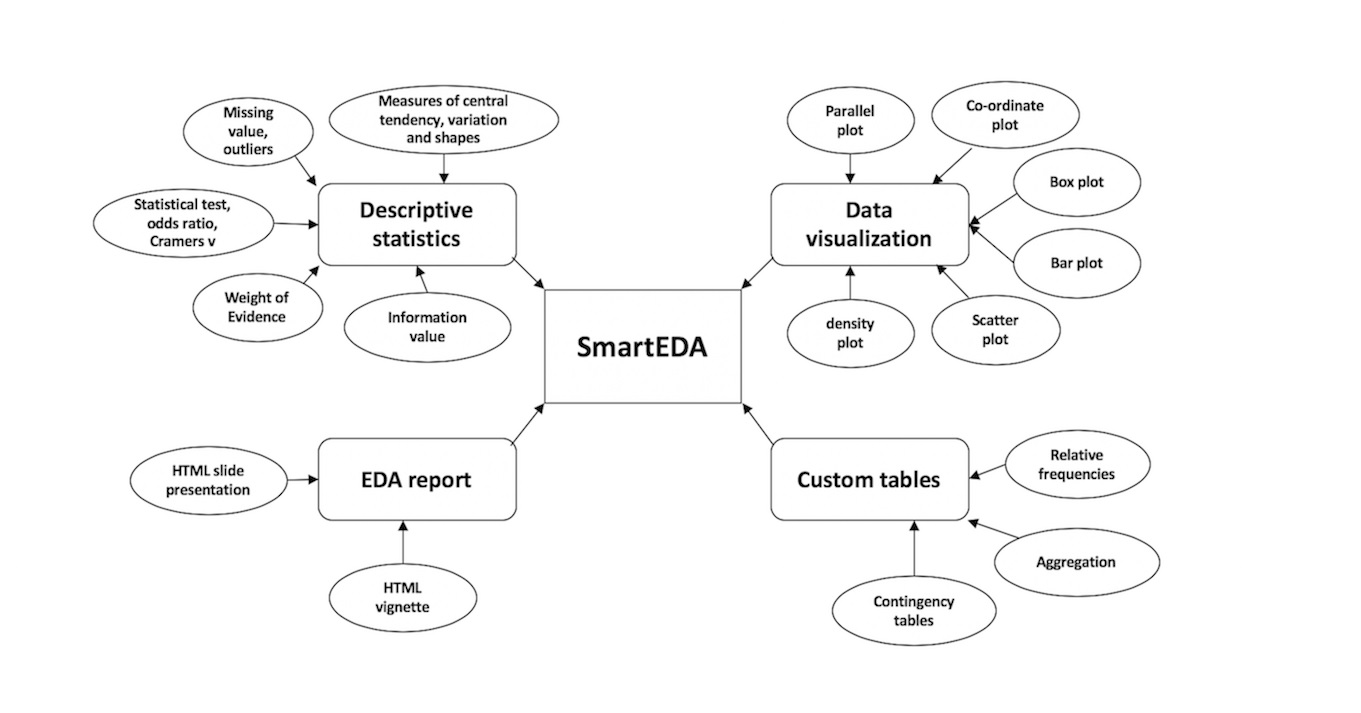
\includegraphics{/Users/jpalbino/Library/Mobile Documents/com~apple~CloudDocs/GitHub/with-a-little-help-from-my-friends/figuras/EDA-Funcionalidades-SmartEDA.jpg}
\caption{Figura 1: As diversas funcionalidades do SmartEDA.}
\end{figure}

\hypertarget{ilustrauxe7uxe3o}{%
\subsubsection{Ilustração}\label{ilustrauxe7uxe3o}}

Aplicamos o SmartEDA para gerar insights sobre as vendas de cadeirinhas
infantis em diferentes localidades.\\
Usaremos os dados ``Carseats'' disponíveis no pacote ISLR (James,
Witten, Hastie, \& Tibshirani, 2017) que contém 11 variáveis, tais como:
vendas unitárias em cada local (Sales); preçocobrado pelos concorrentes
(CompPrice); nível de renda da comunidade (Income); tamanho da população
na região (population); orçamento de publicidade (Advertising), preço
que a empresa cobra pelas cadeirinhas em cada local (Price); qualidade
da localização das prateleiras (ShelveLoc); média idade da população
local (Age), nível educacional em cada local (Education), indicador de
localização urbana/rural Utilizaremos o SmartEDA para entender as
dimensões do conjunto de dados, nomes de variáveis, resumo geral ausente
e tipos de dados de cada variável.

Inicialmente, iremos carregar as bibliotecas SmartEDA e ISLR.

\begin{Shaded}
\begin{Highlighting}[]
\ControlFlowTok{if}\NormalTok{(}\SpecialCharTok{!}\NormalTok{(}\StringTok{"SmartEDA"}\NormalTok{) }\SpecialCharTok{\%in\%} \FunctionTok{installed.packages}\NormalTok{()) }\FunctionTok{install.packages}\NormalTok{(}\StringTok{"SmartEDA"}\NormalTok{)}
\FunctionTok{library}\NormalTok{(SmartEDA)}
\end{Highlighting}
\end{Shaded}

\begin{verbatim}
## Registered S3 method overwritten by 'GGally':
##   method from   
##   +.gg   ggplot2
\end{verbatim}

\begin{Shaded}
\begin{Highlighting}[]
\ControlFlowTok{if}\NormalTok{(}\SpecialCharTok{!}\NormalTok{(}\StringTok{"ISLR"}\NormalTok{) }\SpecialCharTok{\%in\%} \FunctionTok{installed.packages}\NormalTok{()) }\FunctionTok{install.packages}\NormalTok{(}\StringTok{"ISLR"}\NormalTok{)}
\FunctionTok{library}\NormalTok{(}\StringTok{"ISLR"}\NormalTok{)}
\end{Highlighting}
\end{Shaded}

Agora usaremos o SmartEDA para compreender: as dimensões do conjunto de
dados, os nomes e tipos de dados de cada variável e observar um resumo
geral de dados ausentes (missing data) .

\begin{Shaded}
\begin{Highlighting}[]
\NormalTok{Carseats }\OtherTok{\textless{}{-}}\NormalTok{ ISLR}\SpecialCharTok{::}\NormalTok{Carseats}
\FunctionTok{ExpData}\NormalTok{(}\AttributeTok{data=}\NormalTok{Carseats,}\AttributeTok{type=}\DecValTok{1}\NormalTok{)}
\end{Highlighting}
\end{Shaded}

\begin{verbatim}
##                                           Descriptions     Value
## 1                                   Sample size (nrow)       400
## 2                              No. of variables (ncol)        11
## 3                    No. of numeric/interger variables         8
## 4                              No. of factor variables         3
## 5                                No. of text variables         0
## 6                             No. of logical variables         0
## 7                          No. of identifier variables         0
## 8                                No. of date variables         0
## 9             No. of zero variance variables (uniform)         0
## 10               %. of variables having complete cases 100% (11)
## 11   %. of variables having >0% and <50% missing cases    0% (0)
## 12 %. of variables having >=50% and <90% missing cases    0% (0)
## 13          %. of variables having >=90% missing cases    0% (0)
\end{verbatim}

\begin{Shaded}
\begin{Highlighting}[]
\CommentTok{\# saída}
\end{Highlighting}
\end{Shaded}

Agora, vejamos o resumo das variáveis numéricas/inteiras, como
Advertising, Age,CompPrice, Income, Population, Price e Sales.

\begin{Shaded}
\begin{Highlighting}[]
\FunctionTok{ExpNumStat}\NormalTok{(Carseats,}\AttributeTok{by=}\StringTok{"A"}\NormalTok{,}\AttributeTok{gp=}\ConstantTok{NULL}\NormalTok{,}\AttributeTok{Qnt=}\ConstantTok{NULL}\NormalTok{,}\AttributeTok{MesofShape=}\DecValTok{2}\NormalTok{, }\AttributeTok{Outlier=}\ConstantTok{FALSE}\NormalTok{,}\AttributeTok{round=}\DecValTok{2}\NormalTok{,}\AttributeTok{Nlim=}\DecValTok{10}\NormalTok{)}
\end{Highlighting}
\end{Shaded}

\begin{verbatim}
##         Vname Group  TN nNeg nZero nPos NegInf PosInf NA_Value Per_of_Missing
## 4 Advertising   All 400    0   144  256      0      0        0              0
## 7         Age   All 400    0     0  400      0      0        0              0
## 2   CompPrice   All 400    0     0  400      0      0        0              0
## 3      Income   All 400    0     0  400      0      0        0              0
## 5  Population   All 400    0     0  400      0      0        0              0
## 6       Price   All 400    0     0  400      0      0        0              0
## 1       Sales   All 400    0     1  399      0      0        0              0
##         sum min    max   mean median     SD   CV    IQR Skewness Kurtosis
## 4   2654.00   0  29.00   6.64   5.00   6.65 1.00  12.00     0.64    -0.55
## 7  21329.00  25  80.00  53.32  54.50  16.20 0.30  26.25    -0.08    -1.14
## 2  49990.00  77 175.00 124.97 125.00  15.33 0.12  20.00    -0.04     0.03
## 3  27463.00  21 120.00  68.66  69.00  27.99 0.41  48.25     0.05    -1.09
## 5 105936.00  10 509.00 264.84 272.00 147.38 0.56 259.50    -0.05    -1.20
## 6  46318.00  24 191.00 115.80 117.00  23.68 0.20  31.00    -0.12     0.43
## 1   2998.53   0  16.27   7.50   7.49   2.82 0.38   3.93     0.18    -0.10
\end{verbatim}

\begin{Shaded}
\begin{Highlighting}[]
\CommentTok{\#Saída{-} Resumo das variáveis numéricas dos dados Carseats}
\end{Highlighting}
\end{Shaded}

Vamos agora verificar o resumo das variáveis categóricas, ou seja,
ShelveLoc, Urban e US.

\begin{Shaded}
\begin{Highlighting}[]
\FunctionTok{ExpCTable}\NormalTok{(Carseats)}
\end{Highlighting}
\end{Shaded}

\begin{verbatim}
##     Variable  Valid Frequency Percent CumPercent
## 1  ShelveLoc    Bad        96   24.00      24.00
## 2  ShelveLoc   Good        85   21.25      45.25
## 3  ShelveLoc Medium       219   54.75     100.00
## 4  ShelveLoc  TOTAL       400      NA         NA
## 5      Urban     No       118   29.50      29.50
## 6      Urban    Yes       282   70.50     100.00
## 7      Urban  TOTAL       400      NA         NA
## 8         US     No       142   35.50      35.50
## 9         US    Yes       258   64.50     100.00
## 10        US  TOTAL       400      NA         NA
## 11 Education     10        48   12.00      12.00
## 12 Education     11        48   12.00      24.00
## 13 Education     12        49   12.25      36.25
## 14 Education     13        43   10.75      47.00
## 15 Education     14        40   10.00      57.00
## 16 Education     15        36    9.00      66.00
## 17 Education     16        47   11.75      77.75
## 18 Education     17        49   12.25      90.00
## 19 Education     18        40   10.00     100.00
## 20 Education  TOTAL       400      NA         NA
\end{verbatim}

\begin{Shaded}
\begin{Highlighting}[]
\CommentTok{\#Output{-} Resumo das variáveis categóricas dos dados Carseats}
\end{Highlighting}
\end{Shaded}

Podemos visualizar as diferentes representações gráficas usando o pacote
SmartEDA quando aplicado no conjunto de dados ``Carseats''.\\
A Figura 2 mostra as diferentes visualizações gráficas, ou seja, gráfico
de dispersão, gráfico de densidade, gráfico de barras, gráfico de caixa,
gráfico de normalidade e gráfico de coordenadas.

Figura 2: Representações gráficas dos dados Carseats usando SmartEDA

\begin{Shaded}
\begin{Highlighting}[]
\CommentTok{\# Scatter plot}
\FunctionTok{ExpNumViz}\NormalTok{(Carseats,}\AttributeTok{target =} \StringTok{"Price"}\NormalTok{,}\AttributeTok{nlim=}\DecValTok{4}\NormalTok{,}\AttributeTok{fname=}\ConstantTok{NULL}\NormalTok{, }\AttributeTok{col=}\ConstantTok{NULL}\NormalTok{,}\AttributeTok{Page=}\ConstantTok{NULL}\NormalTok{,}\AttributeTok{sample=}\DecValTok{1}\NormalTok{)}
\end{Highlighting}
\end{Shaded}

\begin{verbatim}
## [[1]]
\end{verbatim}

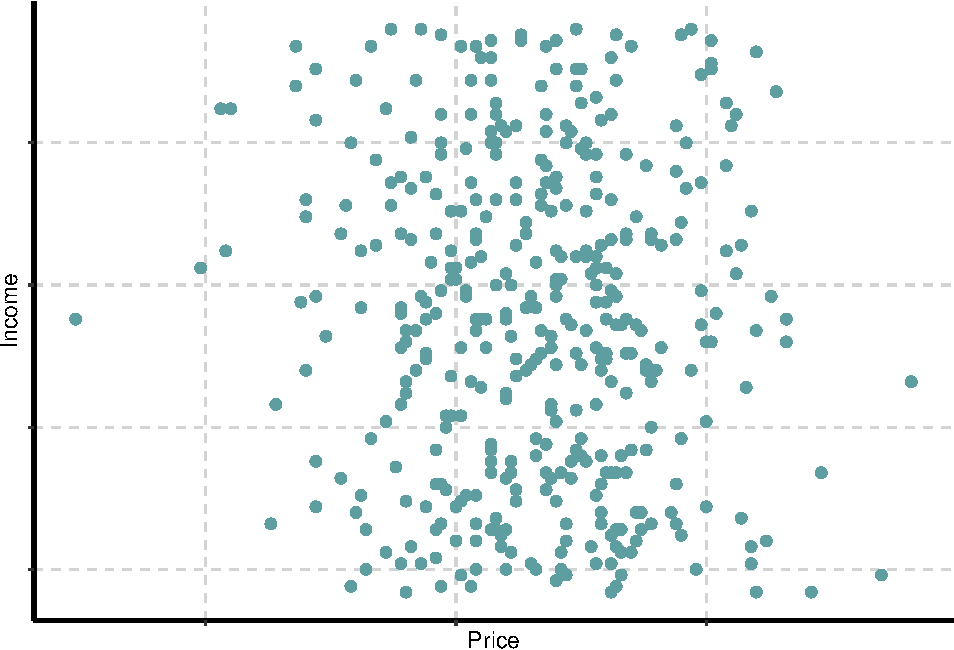
\includegraphics{SmartEDA_osx_files/figure-latex/graficos-1.pdf}

\begin{Shaded}
\begin{Highlighting}[]
\CommentTok{\# Density plot}
\FunctionTok{ExpNumViz}\NormalTok{(Carseats,}\AttributeTok{target=}\ConstantTok{NULL}\NormalTok{,}\AttributeTok{nlim=}\DecValTok{10}\NormalTok{,}\AttributeTok{sample=}\DecValTok{1}\NormalTok{)}
\end{Highlighting}
\end{Shaded}

\begin{verbatim}
## [[1]]
\end{verbatim}

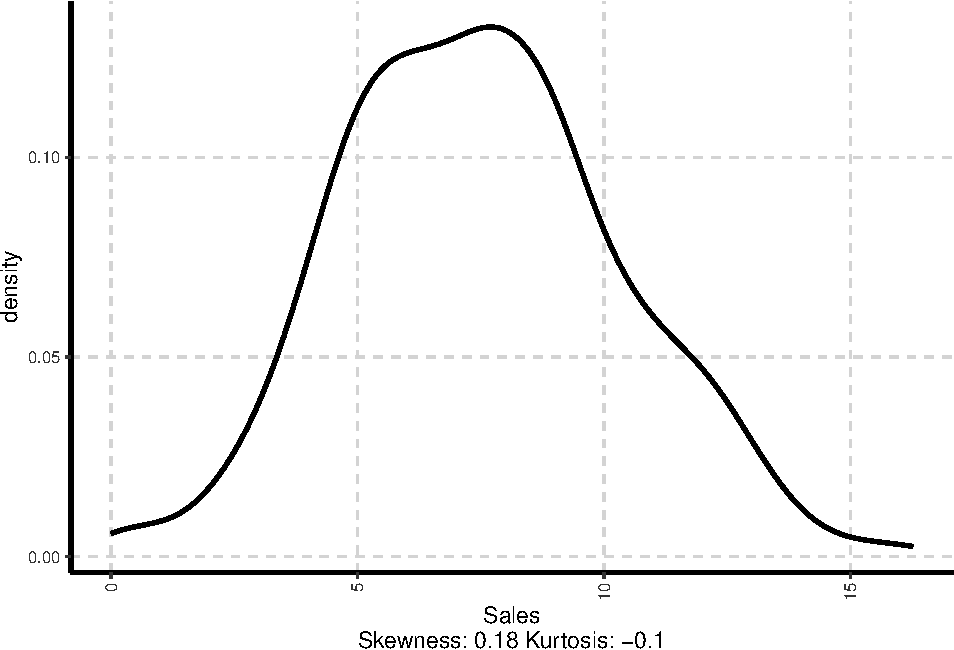
\includegraphics{SmartEDA_osx_files/figure-latex/graficos-2.pdf}

\begin{Shaded}
\begin{Highlighting}[]
\CommentTok{\# Bar plot}
\FunctionTok{ExpCatViz}\NormalTok{(Carseats,}\AttributeTok{target=}\ConstantTok{NULL}\NormalTok{,}\AttributeTok{clim=}\DecValTok{5}\NormalTok{,}\AttributeTok{margin=}\DecValTok{2}\NormalTok{,}\AttributeTok{sample=}\DecValTok{1}\NormalTok{)}
\end{Highlighting}
\end{Shaded}

\begin{verbatim}
## [[1]]
\end{verbatim}

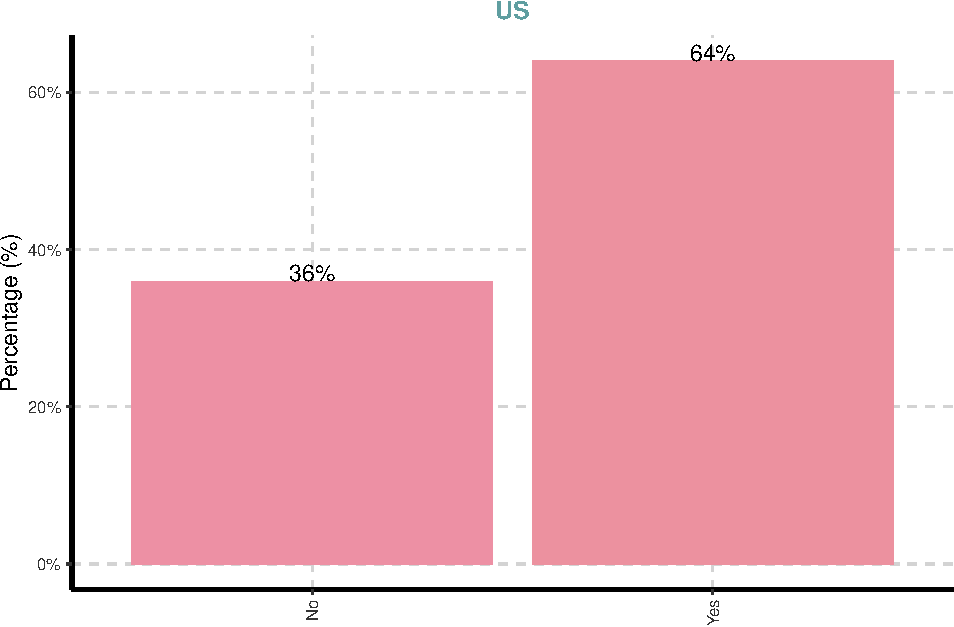
\includegraphics{SmartEDA_osx_files/figure-latex/graficos-3.pdf}

\begin{Shaded}
\begin{Highlighting}[]
\CommentTok{\# Box plot}
\FunctionTok{ExpNumViz}\NormalTok{(Carseats,}\AttributeTok{target=}\StringTok{"US"}\NormalTok{,}\AttributeTok{type=}\DecValTok{2}\NormalTok{,}\AttributeTok{nlim=}\DecValTok{10}\NormalTok{,}\AttributeTok{sample=}\DecValTok{1}\NormalTok{)}
\end{Highlighting}
\end{Shaded}

\begin{verbatim}
## [[1]]
\end{verbatim}

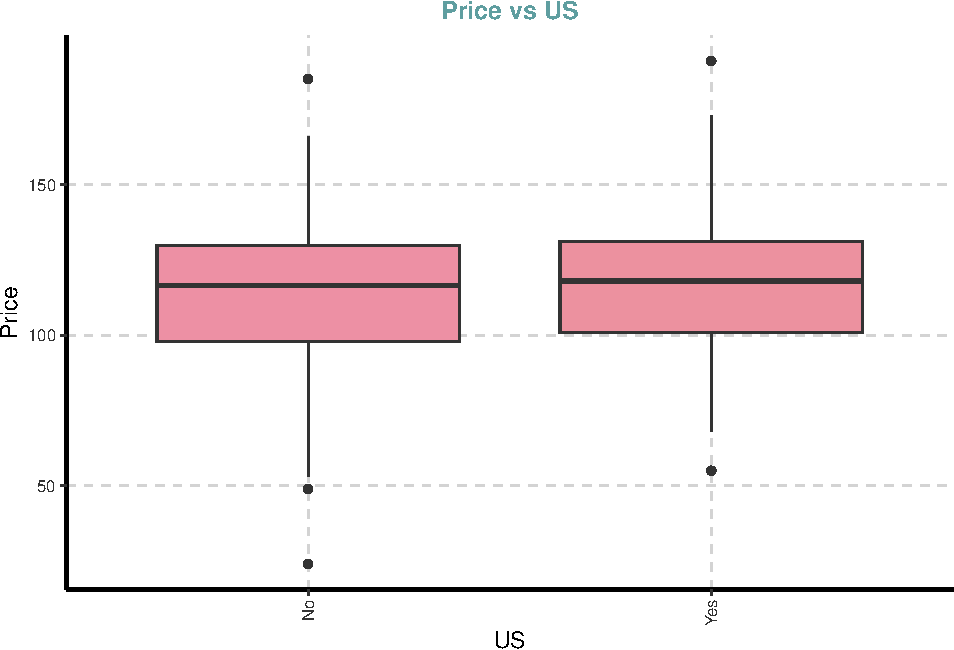
\includegraphics{SmartEDA_osx_files/figure-latex/graficos-4.pdf}

\begin{Shaded}
\begin{Highlighting}[]
\CommentTok{\# Normality plot}
\FunctionTok{ExpOutQQ}\NormalTok{(Carseats,}\AttributeTok{nlim=}\DecValTok{10}\NormalTok{,}\AttributeTok{sample=}\DecValTok{1}\NormalTok{)}
\end{Highlighting}
\end{Shaded}

\begin{verbatim}
## [[1]]
\end{verbatim}

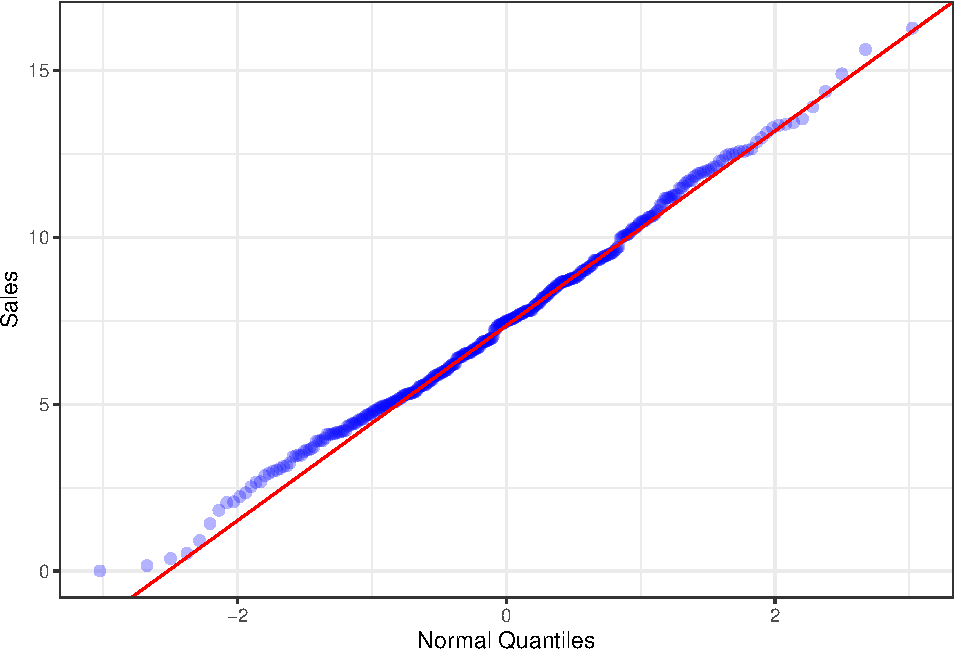
\includegraphics{SmartEDA_osx_files/figure-latex/graficos-5.pdf}

\begin{Shaded}
\begin{Highlighting}[]
\CommentTok{\# Co{-}ordinate plots}
\FunctionTok{ExpParcoord}\NormalTok{(Carseats,}\AttributeTok{Group=}\StringTok{"ShelveLoc"}\NormalTok{,}\AttributeTok{Stsize=}\FunctionTok{c}\NormalTok{(}\DecValTok{10}\NormalTok{,}\DecValTok{15}\NormalTok{,}\DecValTok{20}\NormalTok{),}\AttributeTok{Nvar=}
                 \FunctionTok{c}\NormalTok{(}\StringTok{"Price"}\NormalTok{,}\StringTok{"Income"}\NormalTok{,}\StringTok{"Advertising"}\NormalTok{,}\StringTok{"Population"}\NormalTok{,}\StringTok{"Age"}\NormalTok{,}\StringTok{"Education"}\NormalTok{))}
\end{Highlighting}
\end{Shaded}

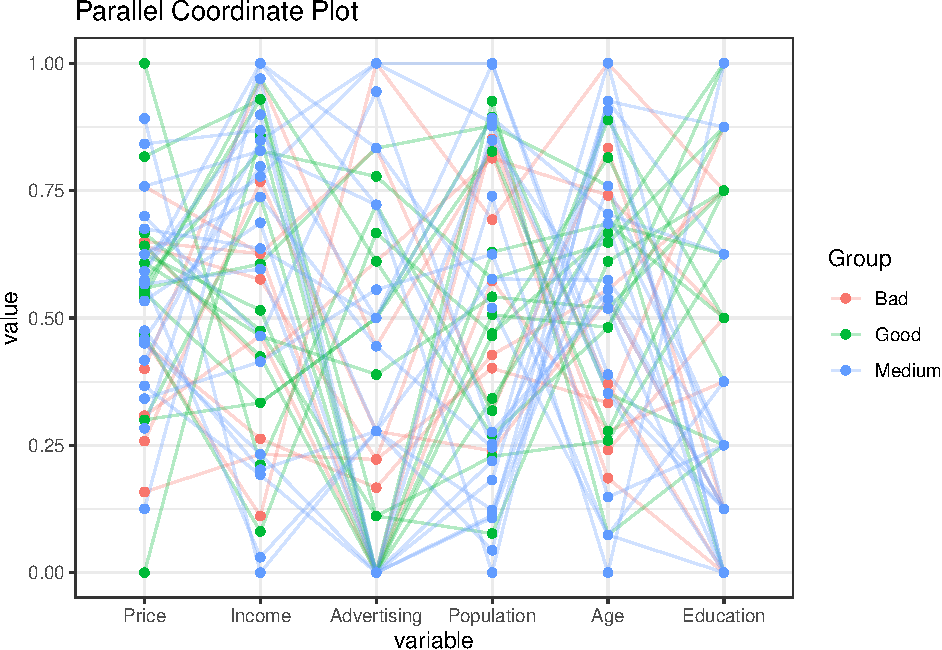
\includegraphics{SmartEDA_osx_files/figure-latex/graficos-6.pdf}

\hypertarget{comparauxe7uxe3o-com-outros-pacotes-r}{%
\subsubsection{Comparação com outros pacotes
R}\label{comparauxe7uxe3o-com-outros-pacotes-r}}

A Figura 3 compara o pacote SmartEDA (Ubrangala, Rama, Kondapalli, \&
Putatunda, 2018) com outros pacotes semelhantes disponíveis no CRAN para
análise exploratória de dados viz.~dlookr (Ryu, 2018), DataExplorer
(Cui, 2018), Hmisc (Harrell et al., 2018), exploreR (Coates, 2016),
Tutor (Nair, 2018) e summarytools (Comtois, 2018).\\
A métrica para avaliação é a disponibilidade de vários recursos
desejados para realizar uma análise exploratória de dados, tais como:\\
(a) Descrever informações básicas para dados de entrada;\\
(b) Função a fornecer;\\
(c) estatísticas resumidas para todas as variáveis numéricas;\\
(d) Função para fornecer gráficos para todas as variáveis numéricas;\\
(e) Função para fornecer estatísticas de resumo para todos os caracteres
ou variáveis categóricas;\\
(f) Função para fornecer gráficos para todos os caracteres ou variáveis
categóricas;\\
(g) Estatísticas de resumo personalizadas - extensão para dados. Pacote
data.table;\\
(h) Gráficos de normalidade/coordenadas;\\
(i) Binarização/binning de recursos;\\
(j) Padronizar/faltar imputação/diagnosticar outliers; e\\
(k) Relatório HTML usando rmarkdown/Shiny.

\begin{figure}
\centering
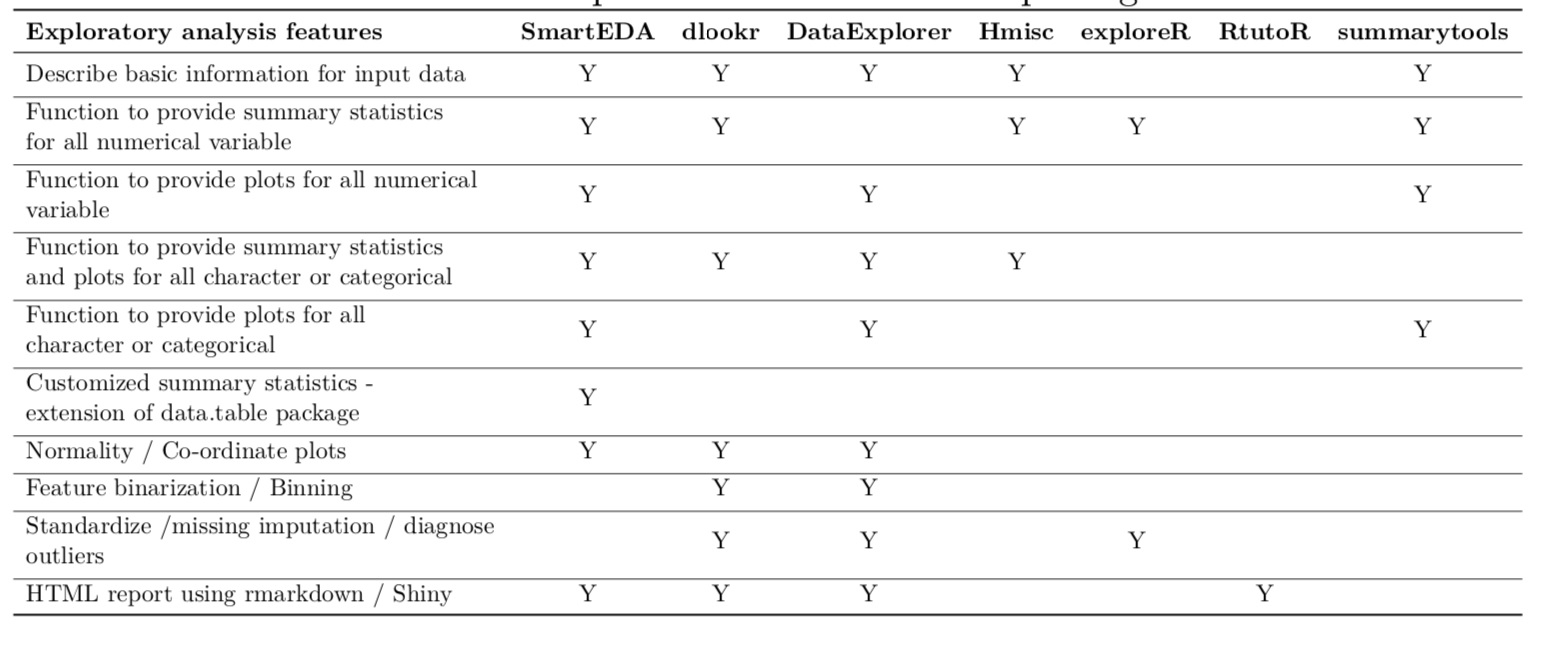
\includegraphics{/Users/jpalbino/Library/Mobile Documents/com~apple~CloudDocs/GitHub/with-a-little-help-from-my-friends/figuras/EDA-Tabela-comparativa-pacotes.jpg}
\caption{Figura 3: Tabela comparativa de pacotes EDA.}
\end{figure}

\hypertarget{conclusuxe3o}{%
\subsubsection{Conclusão}\label{conclusuxe3o}}

A contribuição deste trabalho está no desenvolvimento de um novo pacote
em R ou seja, SmartEDA para Análise Exploratória de Dados
automatizada.\\
O pacote SmartEDA ajuda na implementação da Análise Exploratória de
Dados completa apenas executando a função em vez de escrever um código R
demorado. Os usuários do SmartEDA podem automatizar todo o processo de
EDA em qualquer conjunto de dados com funções fáceis de implementar e
exportar relatórios de EDA que seguem as melhores práticas da indústria
e da academia.\\
O SmartEDA pode fornecer estatísticas resumidas junto com gráficos para
variáveis numéricas e categóricas. Ele também fornece uma extensão para
o pacote data.table que nenhum dos outros pacotes disponíveis no CRAN
oferece.\\
No geral, os principais benefícios do SmartEDA estão na economia de
tempo de desenvolvimento, menor porcentagem de erros e
reprodutibilidade.\\
Em setembro de 2019, o pacote SmartEDA tinha mais de 6.000 downloads, o
que indica sua aceitabilidade e maturidade nas estatísticas e na
comunidade de aprendizado de máquina.\\
Podemos ver na Figura 3 que a versão atual do SmartEDA possui quase
todas as características desejadas mencionadas acima, exceto os pontos
(h) e (i), ou seja, gráficos de normalidade e binning de recursos,
respectivamente. Esses dois recursos seriam incorporados na próxima
versão e estamos trabalhando nisso.\\
No entanto, a funcionalidade exclusiva e mais forte fornecida pelo
SmartEDA é o ponto (f), ou seja, uma extensão para o pacote data.table
que nenhum dos outros pacotes oferece. Assim, o SmartEDA agrega valor
devido à importância e popularidade do data.table entre os usuários do R
para analisar grandes conjuntos de dados.\\
A Figura 3 mostra que o SmartEDA é melhor do que quase todos os outros
pacotes disponíveis no CRAN.\\
O concorrente mais próximo do SmartEDA parece ser o pacote DataExplorer,
mas este não possui os recursos de dataviz (b) e (f). Função para
fornecer estatísticas de resumo para todas as variáveis numéricas e
extensão para dados e para o acote data.table, respectivamente.\\
Além disso, outra característica distintiva que o SmartEDA possui, mas
nenhum dos outros pacotes semelhantes possuem, é a capacidade de
exportar todos os gráficos em um pdf.

\hypertarget{disponibilidade}{%
\subsubsection{Disponibilidade}\label{disponibilidade}}

O software é distribuído sob uma LICENÇA de arquivo MIT + (Repositório:
CRAN) e está disponível em \url{https://github.com/daya6489/SmartEDA}.

\hypertarget{reconhecimentos}{%
\subsubsection{Reconhecimentos}\label{reconhecimentos}}

Queremos agradecer à VMware e à liderança do Enterprise and Data
Analytics (EDA) por nos fornecer a infraestrutura e o suporte
necessários para este trabalho. Somos gratos à comunidade R por sua
aceitação e feedback para melhorar ainda mais nosso pacote.

\hypertarget{referuxeancias-bibliogruxe1ficas}{%
\subsubsection{Referências
Bibliográficas}\label{referuxeancias-bibliogruxe1ficas}}

Chon Ho, Y. (2010). Exploratory data analysis in the context of data
mining and resampling. International Journal of Psychological Research,
3(1), 9--22. \url{doi:https://doi.org/10.21500/} 20112084.819\\
Coates, M. (2016). exploreR: Tools for Quickly Exploring Data. Retrieved
from \{\url{https://CRAN.R-project.org/package=exploreR}\}\\
Comtois, D. (2018). summarytools: Tools to Quickly and Neatly Summarize
Data. Retrieved from
\{\url{https://CRAN.R-project.org/package=summarytools}\}\\
Cui, B. (2018). DataExplorer: Data Explorer. Retrieved from
\{\url{https://CRAN.Rproject}. org/package=DataExplorer\}\\
DiCerbo et al.~(2015). Serious Games Analytics. Advances in Game-Based
Learning. In C. Loh, Y. Sheng, \& D. Ifenthaler (Eds.),. Cham: Springer.
\url{doi:10.1007/978-3-319-05834-4} Harrell et al.~(2018). Hmisc:
Harrell Miscellaneous. Retrieved from \{\url{https://CRAN.Rproject}.
org/package=Hmisc\}\\
James, G., Witten, D., Hastie, T., \& Tibshirani, R. (2017). ISLR: Data
for an Introduction to Statistical Learning with Applications in R.
\url{doi:https://doi.org/10.1007/} 978-1-4614-7138-7\_1\\
Konopka et al.~(2018). Exploratory data analysis of a clinical study
group: Development of a procedure for exploring multidimensional data.
PLoS ONE, 13(8). \url{doi:https://doi.org/10}.
1371/journal.pone.0201950\\
Ma, X., Hummer, D., Golden, J. J., Fox, P. A., Hazen, R. M., Morrison,
S. M., Downs, R. T., et al.~(2017). Using Visual Exploratory Data
Analysis to Facilitate Collaboration and Hypothesis Generation in
Cross-Disciplinary Research. International Journal of Geo-Information,
6(368), 1--11. \url{doi:https://doi.org/10.3390/ijgi6110368}\\
Nair, A. (2018). RtutoR: Shiny Apps for Plotting and Exploratory
Analysis. Retrieved from
\{\url{https://CRAN.R-project.org/package=RtutoR}\}\\
R Core Team. (2017). R: A Language and Environment for Statistical
Computing. Vienna, Austria: R Foundation for Statistical Computing.
Retrieved from \url{https://www.R-project.org/} Ryu, C. (2018). dlookr:
Tools for Data Diagnosis, Exploration, Transformation. Retrieved from
\{\url{https://CRAN.R-project.org/package=dlookr}\}\\
Sande, Gordon (July 2001). ``Obituary: John Wilder Tukey''. Physics
Today. 54 (7): 80--81. \url{doi:10.1063/1.1397408}.\\
Tukey, J. W. (1977). Exploratory data analysis. Addison-Wesley.\\
Ubrangala, D., Rama, K., Kondapalli, R. P., \& Putatunda, S. (2018).
SmartEDA: Summarize and Explore the Data. Retrieved from
\{\url{https://CRAN.R-project.org/package=SmartEDA}\}

\end{document}
